\section{Исследование ресурсоемкости}
\subsection{Общие положения исследования}

Основной целью исследования является построение доверительной
функции ресурсоемкости для рассматриваемого алгоритма. В дальнейшем будем использовать следующее общепринятое определение функции объема памяти (ресурсоемкости) [12, 13]:
\par
\textbf{Определение.} Функция объёма памяти. Под объёмом памяти, требуемым алгоритмом $A$ для входа, заданного множеством $D$, будем понимать максимальное число ячеек памяти информационного носителя модели вычислений, задействованных в ходе выполнения алгоритма.

Функцию объёма памяти алгоритма для входа $D$ будем обозначать через $V_A(D)$. Предполагается, что закон распределения значений $V_A(D)$ неизвестен.

Экспериментально исследование можно разделить на следующие этапы:
\begin{enumerate}
\item Вводится ограниченная дискретная случайная величина с неизвестным распределением.
\item На основе данных, полученных после многократного запуска алгоритма, строится гистограмма относительных частот.
\item Полученная гистограмма аппроксимируется некоторой функцией плотности распределения вероятностей.
\item Для доказательства корректности выбранной функции плотности распределения формулируется и доказывается гипотеза о распределении относительных частот значений функции ресурсоемкости. Если доказать гипотезу не удалось, необходимо выбрать другую функцию и повторить данный шаг.
\item После того, как гипотезу удалось доказать, для функции нужно выбрать коэффициент доверия $\gamma$.
\item Далее решается интегральное уравнение и находится значение $V_{\gamma}(n)$ ресурсоемкости.
\end{enumerate}

Найденное на последнем шаге значение и есть доверительная ресурсоемкость алгоритма. Его можно интерпретировать так: для единичного входа алгоритма, его ресурсоемкость будет заключена в сегмент $[V^{\vee}, V_{\gamma}]$, т. е. между лучшим случаем и значением $V_{\gamma}(n)$ с вероятностью $\gamma$.

\subsection{Построение гистограммы частот}

Перед построение гистограммы относительных частот необходимо нормировать данные. Введем случайную нормированную величину $T$. Ее реализации $t_i$ получаются на основе теоретических и эмпирических значений ресурсоемкости [8]:
$$t_i = \frac{V_i - V^{\vee}}{V^{\wedge} - V^{\vee}}$$
где $V_i$ — значение функции ресурсоемкости для сгенерированных случайных допустимых входов $D_i$: $V_i = V_A(D_i)$, $i = \overline{1, m}$, а $V^{\wedge}, V^{\vee}$ — теоретический максимум и минимум функции объема памяти соответственно. При этом отметим, что
нормированные величины $t_i$ принимают значения из сегмента [0, 1].

Далее необходимо определить количество полусегментов для построения гистограммы относительных частот. Существует множество способов это сделать. Воспользуемся эмпирическим правилом:
$$k = [\sqrt{n}],$$
где $n$ — общее число наблюдений.

\subsection{Определение объема выборки}

Для построения гистограммы относительных частот нужно определить размер выборки. Заметим, что не всегда имеется возможность проводить повторные эксперименты и исследователи вынуждены работать с уже полученными данными. Такое ограничение может быть связано с несколькими факторами, например, дороговизной или трудоемкостью. Но даже когда возможность проводить эксперименты есть, имеет смысл минимизировать размер выборки для сокращения дополнительных расходов. Возникает проблема определения минимального числа экспериментов $m$ для вычисления ресурсоемкости алгоритма при заданной доверительной вероятности $\gamma$. Заметим, что длина входа $n$ при этом остается постоянной.

\subsubsection{Метод с использованием схемы Бернулли}
При известной вероятности $p$ значений трудоемкости с наименьшей
частотной встречаемостью можно применить метод на основе схемы Бернулли [12]. Его суть заключается в том, что величина $p$ трактуется как
вероятность успеха и рассматривается событие $A$ — наблюдение как минимум одного успеха в $m$ испытаниях с заданной вероятностью $\gamma$. Сама
задача сводится к определению числа испытаний $n$ в схеме Бернулли:

$$P(A) = 1 - (1 - p)^m \geq \gamma,$$
\noindentоткуда можно получить требуемый объем выборки:

$$m \geq \ceil*{ \frac{ln(1 - p)}{ln(1 - \gamma)}}$$

\subsubsection{Метод на основе закона распределения}

Более общий метод основан на рассмотрении гипотезы о законе распределения функции трудоемкости алгоритма [9]. Поскольку закон распределения значений $V_A(D)$ неизвестен, вводится гипотеза, что значения функции трудоемкости являются ограниченной дискретной случайной величиной, которая распределена по одному из хорошо известных законов распределения. Суть данного метода сводится к тому, что для определения минимального объема выборки $m$ проводится ряд последовательных экспериментов с постоянной длиной входа $n$. Значение $n$ задается исследователями, как и начальный объем выборки $m$.

На каждой итерации извлекаются выборки размера $m$ и вычисляются значения ресурсоемкости. Далее рассчитывается ряд статистических величин: выборочное среднее $\overline{V_{\epsilon}}(m)$ и выборочная исправленная дисперсия $S^2$ , которые являются оценками теоретической ресурсоемкости $\overline{V_A}$ и теоретической дисперсии ресурсоемкости $\sigma^2_A$ соответственно. Требуемый объем выборки рассчитывается по формуле:

$$m^* = m^*(\delta, \gamma) = min m : P(|\overline{V_{\epsilon}}(m) - \overline{V_A}|) \leq \delta) \leq \gamma,$$

\noindentт. е. минимальный объем выборки нужно выбирать таким образом, чтобы средние значения в выборке $\overline{V_{\epsilon}}$ позволяли построить доверительный интервал длиной $2\delta$, который покрывал бы неизвестное значение $\overline{V_A}$ с надежностью $\gamma$.
При этом условием останова для описанной последовательности итераций является выполнение неравенства:

$$m^*_{(i+1)} < m^*_{(i)},$$

\noindentгде $m^*_{(i)}$ — рассчитанный минимальный объем выборки на итерации $i$.

\pagebreak
\section{Проведение экспериментального исследования функции объема памяти}
\subsection{Описание выбранного алгоритма}

Проводить анализ на ресурсоемкость имеет смысл для алгоритмов с неконстантным использованием дополнительной памяти. Например, алгоритм сортировки, который работает <<на месте>>, не подойдет т. к. размер дополнительной памяти будет равен или очень близко равен 0 вне зависимости от входа алгоритма. Подойдут алгоритмы, использующие такие структуры данных как stack, deque, queue. Простейший пример такого алгоритма --- Обход в ширину, который использует очередь для обхода графа.

Для исследования был выбран алгоритм Левита [14]. Этот алгоритм находит кратчайшие пути от одной вершины до всех остальных на графах без петель. Стоит отметить, что алгоритм Левита работает даже на графах, где существуют ребра отрицательного веса, но при этом не должно существовать отрицательных циклов.

Входными данными для алгоритма является граф $G$, представленный в виде упорядоченной совокупности множеств вершин $V$ и ребер $E$:
$G = (V, E)$. Оценка размера входных данных производится по размеру
множеств вершин и ребер. Пусть $n$ — количество вершин в множестве $V$, $m$ — количество ребер в множестве $E$: $n = |V|$, $m = |E|$. В качестве размера дополнительной памяти будем брать максимальный размер дэка, который будет зафиксирован во время выполнения алгоритма.

\subsection{Генерация данных}

Нужно генерировать связные ориентированные графы с $n$ вершинами и $m$ ребрами. Количество ребер возьмем $m = 10n$. В общем случае $n$  и $m$ будут зависеть от поставленной задачи.

Для генерации связного графа с $m$ ребрами воспользуемся следующим алгоритмом:
\begin{enumerate}
\item Сначала построим дерево. Для этого соединим вершину $i$ с вершиной $(i + 1)$, для $i = \overline{1, n-1}$.
\item $m - n - 1$ раз соединим две случайные вершины.
\end{enumerate}

Этот алгоритм будем использовать как для предварительного, так и для основного исследования.

\subsection{Этап предварительного исследования}

Выдвигается гипотеза, что функция ресурсоемкости алгоритма Левита имеет бета-распределение. Основные шаги предварительного исследования:

\begin{enumerate}
\item Фиксация значения длины входа $n = 1000$ из сегмента длин в области применения алгоритма.

\item Определение необходимого числа экспериментов $m = 10000$ (объем выборки).

\item Проведение экспериментального исследования и получение значений
ресурсоемкости $V_i$ для сгенерированных случайных допустимых входов $D_i: V_i = V_A (D_i), i = \overline{1, m},$

где $D_i$ - случайный допустимый вход, $V_A$ - алгоритм Левита.

Значение ресурсоемкости берется как максимальный размер очереди за время выполнения всего алгоритма.

\item Получение теоретических функций ресурсоемкости алгоритма для лучшего и худшего случаев. Функции $V_{A}^{\vee}$ и $V_{A}^{\wedge}$ для алгоритма Левита имеют вид:

$$V_{A}^{\vee}(n) = 1$$
$$V_{A}^{\wedge}(n) = n$$

Худший случай обоснован тем, что в любой момент времени в очереди находится не больше 1 вершины $v_i$. Вершин всего $n$, следовательно в очереди может находиться не более $n$ элементов.

\item Выбор числа $k = 100$ полусегментов для гистограммы относительных частот значений ресурсоемкости.

Значение $k$ получено через эмпирическое правило $$k = \sqrt{m}$$

\item Вычисление нормированного выборочного среднего и нормированной
исправленной выборочной дисперсии по формулам [9]:

$$\overline{t} = \frac{\overline{V_{t}}(n)- V^{\vee}}{V^{\wedge} - V^{\vee}}$$

$$s^2 = \frac{1}{m - 1} \sum\limits_{i=1}^m \frac{(V_i - \overline{V_t}(n))^2}{(V^{\wedge} - V^{\vee})^2}$$

где $V^{\wedge}$ и $V^{\vee}$ — соответственно максимальное и минимальное значение теоретических функций ресурсоемкости, $\overline{V_{t}}(n)$ — выборочное среднее.

\item Формулировка гипотезы об аппроксимирующем законе распределения и расчет параметров этого закона. В рассматриваемом случае
выдвигается гипотеза о бета-распределении.

Напомним, что случайная величина $X$ имеет бета-распределение, если она задаётся плотностью вероятности $V_X$, имеющей вид:

$$V_X(x) = \frac{1}{B(\alpha, \beta)}x^{\alpha - 1}(1 - x)^{\beta - 1},$$
где
 \begin{itemize}
\item $\alpha, \beta > 0$ произвольные фиксированные параметры, и
\item $B(\alpha, \beta) = \int_{0}^{1}x^{\alpha - 1}(1 - x)^{\beta - 1}dx$ — бета-функция.
\end{itemize}

Параметры бета-распределения рассчитываются по формулам [9]:

$$\alpha = \frac{\overline{t}}{s^2} (\overline{t} - (\overline{t})^2 - s^2)$$

$$\beta = \frac{(1 - \overline{t}}{s^2} (\overline{t} - (\overline{t})^2 - s^2)$$

В данном случае $\alpha = 2817, \beta = 677$.

\item Расчет теоретических частот по формуле функции плотности [9]:

$$p_i = \int_{x_i}^{x_i + \Delta x_i}  b(x, \alpha, \beta) dx,$$

где $b$ — функция бета-распределения.

\item Расчет наблюдаемого значения критерия согласия Пирсона по формуле [15]:

$$\chi ^2_{\text{набл}} = m \sum\limits_{i=1}^s \frac{(w_i - p_i)^2}{p_i},$$

где $w_i$ — относительные частоты.

\item Проверка гипотезы о законе распределения: если нулевая гипотеза
принимается, то осуществляется переход к основному этапу исследования. Иначе —
выбор другого закона распределения и повтор шагов 8–11.

В данном случае $\chi^2_{\text{набл}} = 109$, а $\chi^2_{\text{кр}} = 124$ (вычислено стандартной функцией пакета Microsoft Excel). Так как $\chi^2_{\text{набл}} < \chi^2_{\text{кр}}$, то нулевая гипотеза принимается.

\end{enumerate}

На рисунке 2 представлена гистограмма относительных частот, а так же аппроксимирующая ее функция.

\begin{figure}[h!]
\center{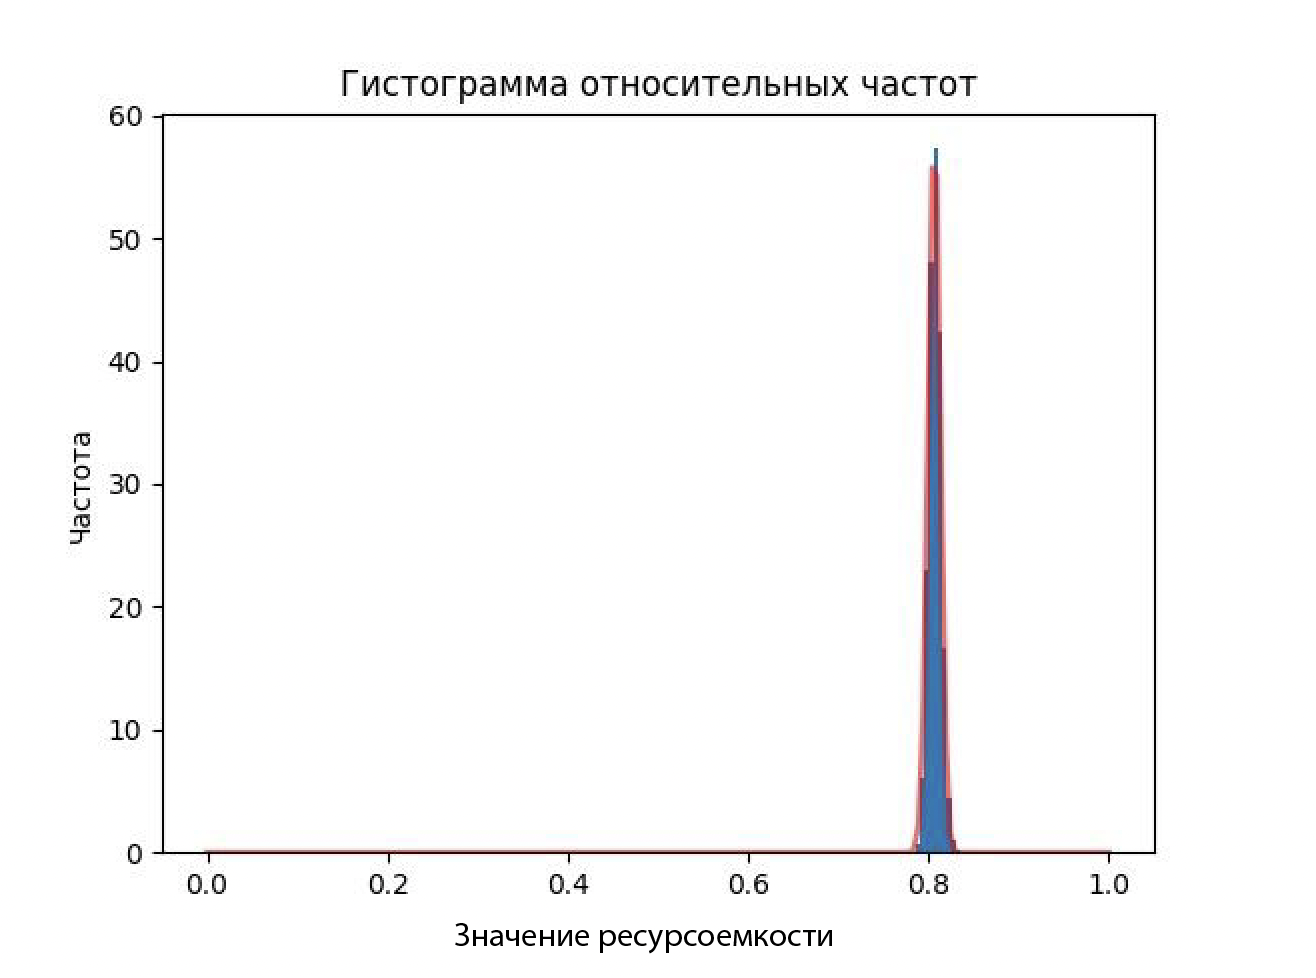
\includegraphics[width=0.7\linewidth]{images/gist.png}}
\caption{Теоретические и эмпирические частоты для алгоритма Левита при $n = 1000$ с разбиением нормированного сегмента $[0, 1]$ на 100 полусегментов}
\label{ris:image1}
\end{figure}

\subsection{Этап основного исследования}

Задача этапа основного исследования — построение функции доверительной ресурсоемкости на основе данных, полученных из экспериментального исследования.

\begin{enumerate}
\item Определение сегмента значений длин входа. В рассматриваемом случае алгоритма Левита будет применяться для графов с количеством вершин от 100 до 1400;

\item Выбор шага изменения длины входа для сегмента. Данный
шаг будет использоваться для проведения экспериментального исследования. В рассматриваемом случае значение шага равно 100;

\item Определение необходимого числа $m$ экспериментов с программной
реализацией алгоритма для фиксированной длины входа. В данном случае $m = 10000$. По итогам экспериментального исследования определяется выборочная средняя и дисперсия. 

\item Расчет на основе данных, полученных из экспериментального исследования, выборочной средней и дисперсии для каждого значения $n$.

\item Расчет на основе результатов, полученных на шаге 4, параметров
аппроксимирующего бета-распределения по формулам из прошлого раздела как
функций длины входа $\alpha(n)$, $\beta(n)$;

\item Определение значения коэффициента доверия и вычисление значений левого $\gamma$-квантиля бета-распределения [12]:

$$\delta_{I, Q}(\gamma) = B^{-1}(\frac{1}{2} + \frac{\gamma}{2}, \alpha, \beta) - B^{-1}(\frac{1}{2} - \frac{\gamma}{2}, \alpha, \beta)$$

\item Вычисление значений функции доверительной ресурсоемкости для исследуемого сегмента длин входа по формуле [8]:

$$V_{\gamma}(n) = V^{\vee}(n) + x_{\gamma}(n)(V^{\wedge} - V^{\vee})$$

\end{enumerate}


\begin{figure}[h!]
\center{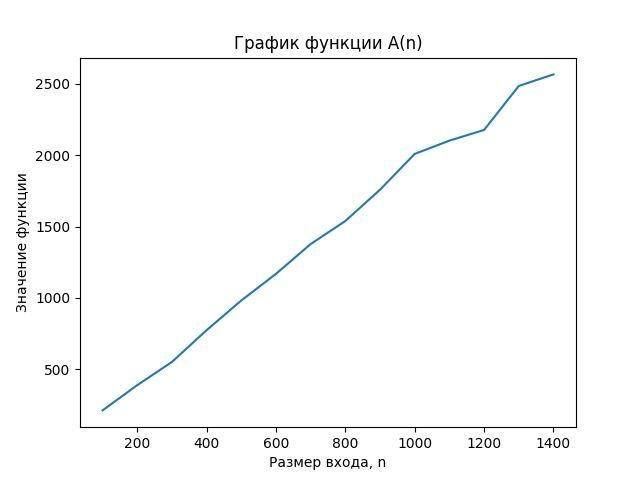
\includegraphics[width=0.7\linewidth]{images/2.jpeg}}
\caption{График функции $\alpha(n)$ — параметра $\alpha$ аппроксимирующего бета-распределения для алгоритма Левита}
\label{ris:image1}
\end{figure}

\begin{figure}[h!]
\center{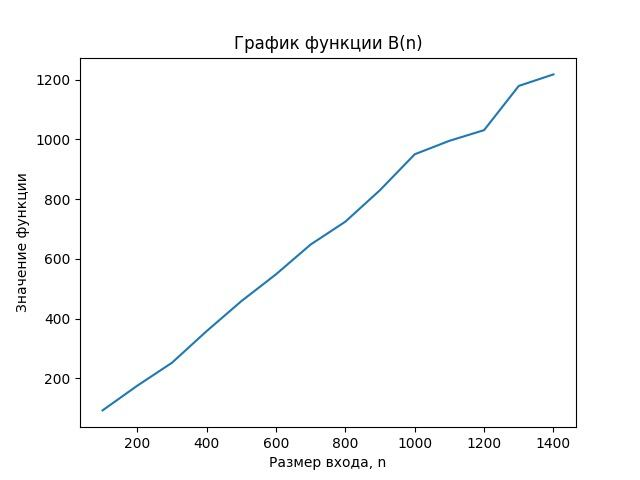
\includegraphics[width=0.7\linewidth]{images/3.jpeg}}
\caption{График функции $\beta(n)$ — параметра $\beta$ аппроксимирующего бета-распределения для алгоритма Левита}
\label{ris:image1}
\end{figure}
\newpage
\begin{figure}[h!]
\center{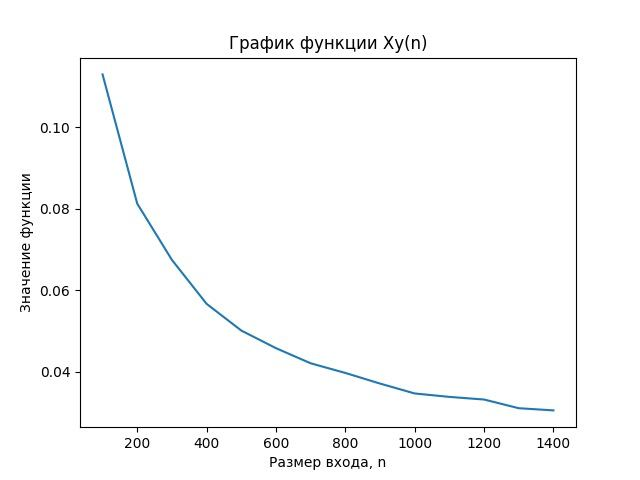
\includegraphics[width=0.7\linewidth]{images/4.jpeg}}
\caption{График зависимости левого $\gamma$-квантиля бета-распределения $x_{\gamma}(n)$ от длины входа для алгоритма Левита}
\label{ris:image1}
\end{figure}

\begin{figure}[h!]
\center{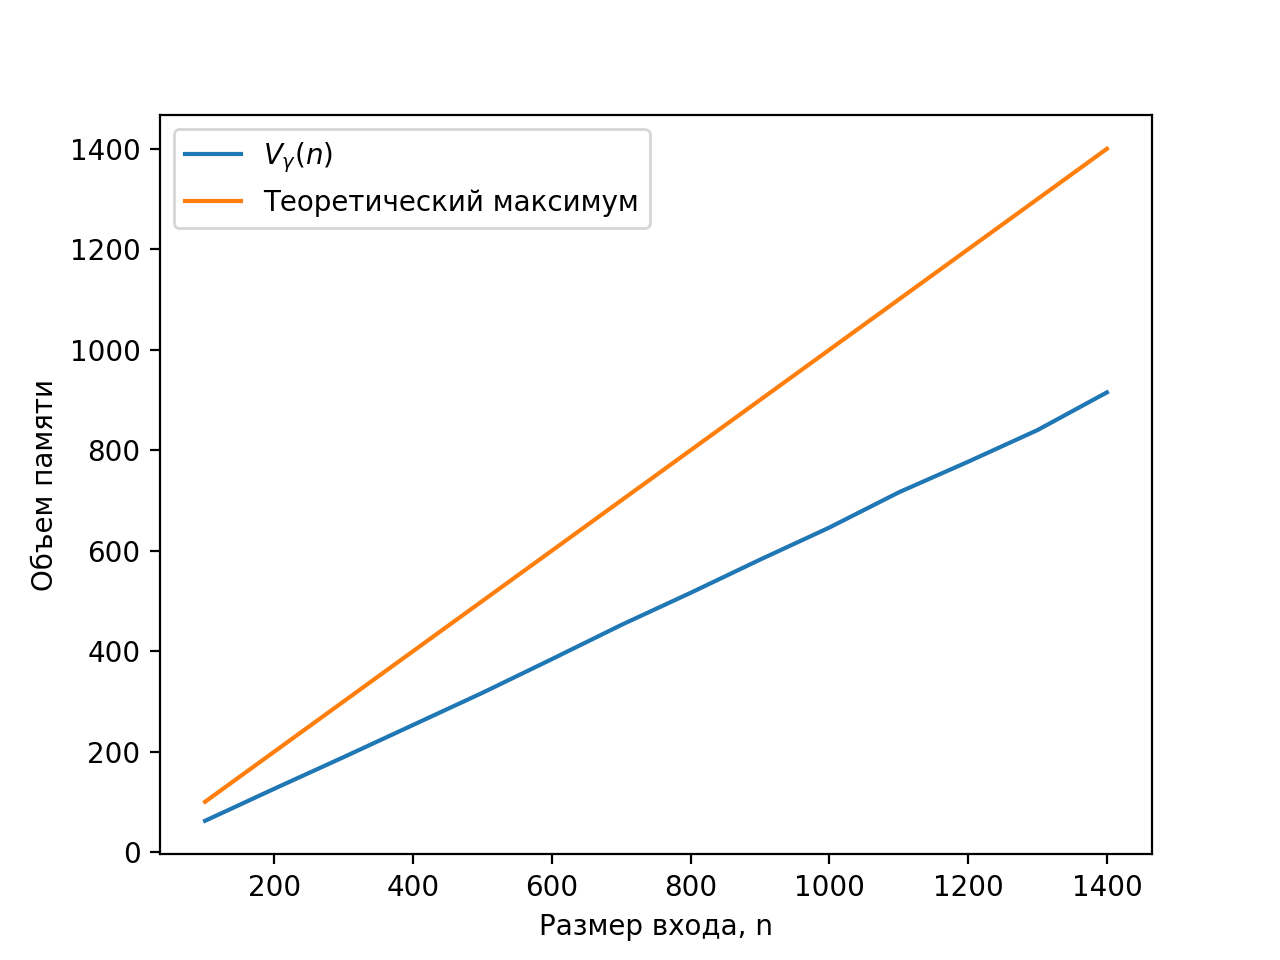
\includegraphics[width=0.7\linewidth]{images/general.png}}
\caption{График доверительной ресурсоемкости и ресурсоемкости в худшем случае для алгоритма Левита}
\label{ris:image1}
\end{figure}

\pagebreak
\section{Создание автоматизированной системы}

Система должна быть легкой и понятной в использовании, доступной, а также должна быть написана на общеизвестных языках программирования. Последний пункт необходим, для дальнейшей модернизацией системы со стороны исследователей и разработчиков.

Был разработан web-сайт --- такое решение не требует установки приложений на устройства. Сайт позволяет загружать данные работы алгоритма, после этого проводит анализ и выгружает результаты на страницу.

В качестве стека технологий для разработки сайта были выбраны:\\
• Бэкенд
\par
--- NGINX --- веб-сервер, работающий на Unix-подобных операционных системах. Был использован, так как имеет ряд преимуществ: малый размер, масштабируемость, простота конфигурации, активная поддержка сообщества, хорошую документацию.
\par
--- Flask --- микрофреймворк для создания веб-приложений написанный на языке программирования Python. Микрофреймворк по размеру является небольшим решением и служит как базовый инструментарий, не реализуя ничего лишнего. Тем не менее, этого достаточно для данной работы. Был использован для реализации основных функции API для сбора, обработки и анализа.

\noindent• Фронтенд
\par
--- JavaScript --- мультипарадигменный язык программирования, был создан для того, чтобы делать веб-страницы <<живыми>>. Программы написанные на этом языке именуются скриптами. Позволяют использоваться в HTML и выполняются при загрузке веб-страницы автоматически. Среди языков для разработки интерфейсов в браузере является распространённым решением.
\par
--- AJAX --- аббревиатура от Asynchronous JavaScript and XML. С помощью этой технологии представляется возможным обмен данными браузера с сервером в <<фоновом>> режиме. В результате такого принципа веб-страница не перезагружается полностью при обновлении данных. Таким образом, веб-приложения становятся быстрее и удобнее.

\begin{figure}[h!]
\center{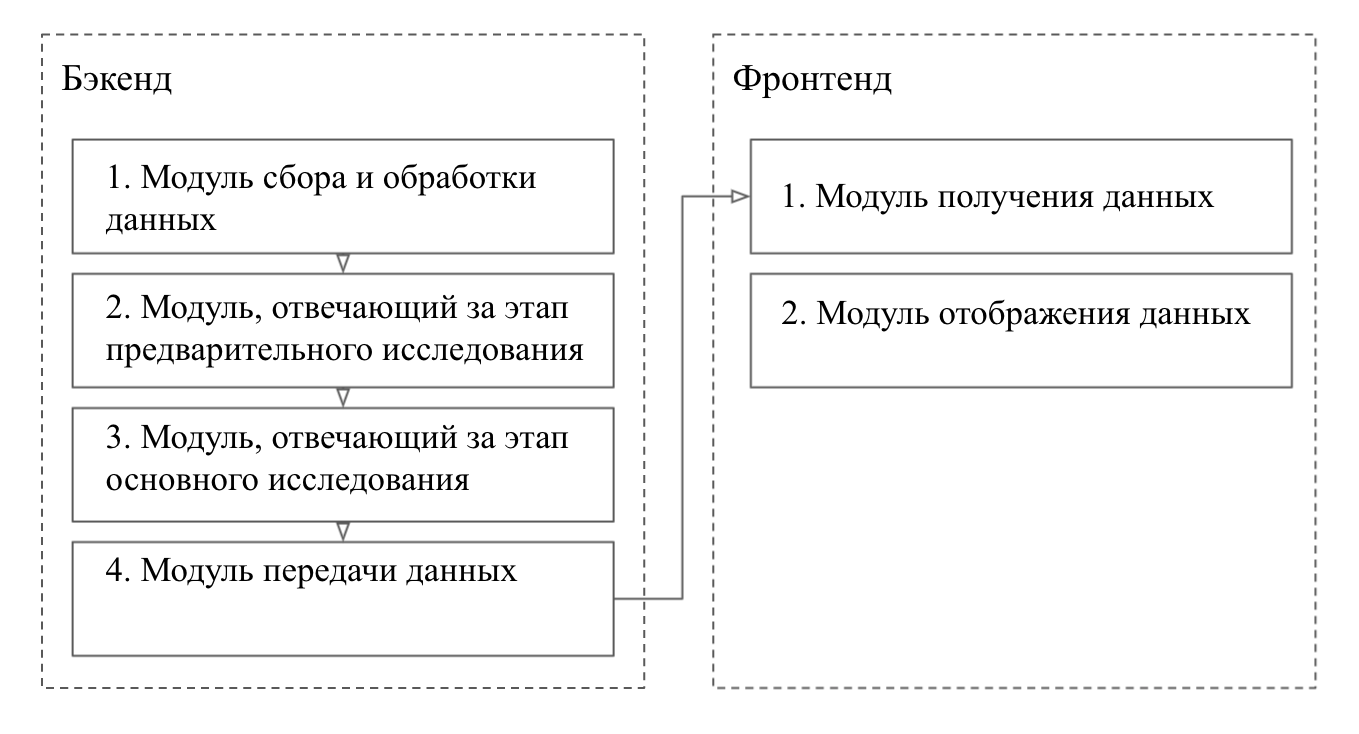
\includegraphics[width=1\linewidth]{images/architecture.png}}
\caption{Архитектура программной реализации}
\label{ris:image1}
\end{figure}

\pagebreak